\section{Project Management Review}
\subsection{Current progress}

During the initial stages of the project, time was dedicated to researching the appropriate language to use, the file format and the methods and algorithms used by other packages. This involved looking at the projects done in the field of music in Python previously, such as Music21 \parencite{Music21}, and other projects listed on the Python Foundation website \parencite{pmus}. 

Many important decisions were made from this research period, such as the decision to use Lilypond to typeset music files rather than create a new algorithm and the research of MusicOCR options available, leading to the decision that MusicOCR is too big a topic for this project to create a new algorithm.


After this research period, class diagrams were drawn and some initial code implementation for the rendering and metadata objectives was developed. It was decided after this initial stage to use Test Driven Development, as the code base and algorithm for loading in a music file was becoming hard to confirm crucial details were being parsed correctly. A set of unit tests were written for the initial implementation, and from this point onward the methodology was applied.

\begin{figure}[h]
    \centering
    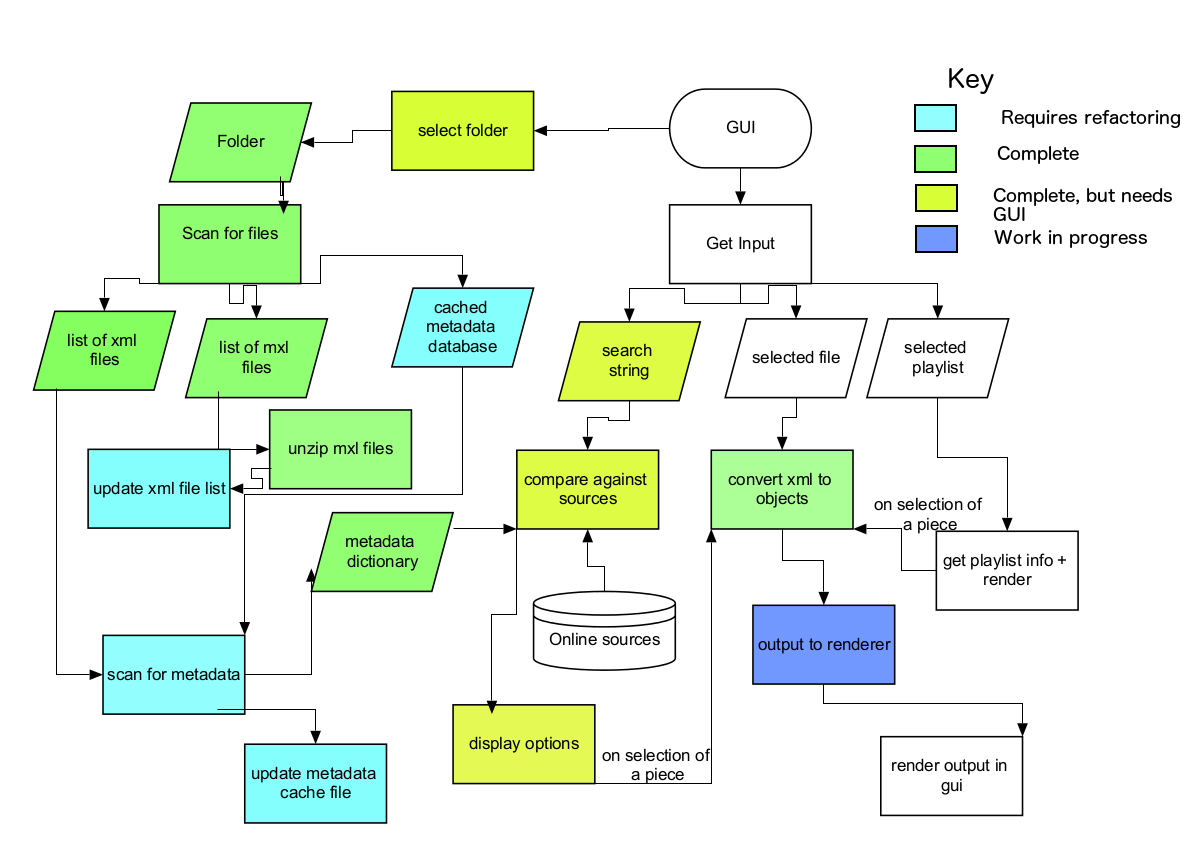
\includegraphics[width=420pt]{flowchart-progress.png}
    \caption{Flowchart colour coded according to progress}
    \label{fig:colours}
\end{figure}
Figure \ref{fig:colours} shows the flowchart shown in figure \ref{fig:flow} colour coded to show progress. Green indicates that this area is considered complete, light blue indicates that this area has been completed but requires refactoring, yellow indicates that this area has been implemented on a command-line level but requires connection to a user interface to be considered completed, and dark blue indicates the area currently in development.

Of the areas shaded in light blue, the cached metadata database is currently stored as a serialised python object. In order to make this as extendible and portable as possible, this will need to be refactored to using an SQLite file to be considered completed. SQLite is a light implementation of an SQL database stored as a single file, which should be relatively simple to implement in other languages as it is standardised.
\subsection{Adjustments made}
During the initial planning phase the developer included coursework deadlines. However, concessions were not considered at times when these courseworks should and did take precedence. In particular, the week before the Languages and Compilers coursework deadline work was solely focussed on development for this coursework.

Furthermore, the intial research phase was very open ended and some topics took less time than was intended than others. In this case, the developer used the extra time working on other courseworks, though in the future adjustments to move future tasks forward should be done instead.

Thirdly, the development methodology in use now is Test Driven Development, meaning that the testing phases between prototype developments can be changed to specified testing sections, such as user interface testing and stress testing, rather than functionality testing.

Finally, the first two weeks of term were affected by jetlag from attending a conference in the United States, which meant that documentation and development suffered a little. Again, the developer was aware that this could occur and should have considered it as a potential risk, though this particular problem will not occur again in the course of the project.

Considering these factors, the revised timeplan in figure \ref{fig:timeplan} includes time dedicated solely to the two final courseworks for other modules and attempts to more clearly define tasks which are open ended, therefore may take a shorter amount of time than predicted.

\begin{landscape}
\subsection{Revised timeplan}
\begin{figure}[H]
	\centering
  \fbox{
   \scalebox{0.3}{\includegraphics*[viewport=0 2538 1892 3808]{timeplan}}
  }
\end{figure}
\begin{figure}[h]
\centering
 \fbox{
   \scalebox{0.3}{\includegraphics*[viewport=0 1269 1892 2538]{timeplan}}
  }
\end{figure}
\begin{figure}[h]
\centering
  \fbox{
   \scalebox{0.3}{\includegraphics*[viewport=0 0 1892 1269]{timeplan}}
  }
 \caption{Updated timeplan}
 \label{fig:timeplan}
\end{figure}
\end{landscape}
